\documentclass[12pt]{article}

%\documentclass[17pt]{extarticle}

%\usepackage{extsizes}
\usepackage{indentfirst}
\usepackage[utf8x]{inputenc}
\usepackage[T1]{fontenc}
\usepackage[english,lithuanian]{babel}
\usepackage{array}
\usepackage{caption}
\usepackage{makecell}
\usepackage[euler]{textgreek}

\usepackage{amsmath, amsthm, amssymb}
\usepackage{graphicx}
\usepackage{setspace}
\usepackage{verbatim}
\usepackage[left=3cm,top=2cm,right=1.5cm,bottom=2cm]{geometry}

\onehalfspacing

\newcommand{\EE}{\mathbb{E}\,} % Mean
\newcommand{\ee}{{\mathrm e}}  % nice exponent
\newcommand{\dd}{{\mathrm d}}
\newcommand{\RR}{\mathbb{R}}

\begin{document}
\selectlanguage{lithuanian}

\begin{titlepage}
\vskip 20pt
\begin{center}

\includegraphics[scale=0.5]{MIF}
\end{center}

%%%%%%%%%%%%%%%%%%%%%%%%%%%%%%%%%%%%%%%%
% TITULINIO PUSLAPIO TEKSTAS
%%%%%%%%%%%%%%%%%%%%%%%%%%%%%%%%%%%%%%%%

\vskip 20pt
\centerline{\bf \large \textbf{VILNIAUS UNIVERSITETAS}}
\bigskip
\centerline{\large \textbf{MATEMATIKOS IR INFORMATIKOS FAKULTETAS}}
\bigskip
\centerline{\large \textbf{BIOINFORMATIKOS BAKALAURO STUDIJŲ PROGRAMA}}

\vskip 90pt
\begin{center}
    {\bf \LARGE \emph{tbx5} ir \emph{tcf21} genų įtakos regeneracijai tyrimai}
\end{center}
\begin{center}
    {\bf \Large Research of the \emph{tbx5} and \emph{tcf21} genes' functions in regeneration}
\end{center}
\vskip 20pt
\centerline{\bf \large \textbf{Kursinis darbas}}
\bigskip
\vskip 50pt

\hskip 140pt {\large Autorius: Danielė Stasiūnaitė}

\hskip 140pt{\large VU el. p.: (daniele.stasiunaite@mif.stud.vu.lt)}
\bigskip
\vskip 20pt

\hskip 140pt {\large Darbo vadovas: J. Asist. Kotryna Kvederavičiūtė}
\vskip 60pt
\vskip 60pt
\centerline{\large \textbf{Vilnius}}
\centerline{\large \textbf{2022}}
\newpage
\end{titlepage}

\selectlanguage{lithuanian}

%%%%%%%%%%%%%%%%%%%%%%%%%%%%%%%%%%%%%%%%
% TURINIO PUSLAPIS
%%%%%%%%%%%%%%%%%%%%%%%%%%%%%%%%%%%%%%%%  
\tableofcontents
\newpage

%%%%%%%%%%%%%%%%%%%%%%%%%%%%%%%%%%%%%%%%
% LIETUVIŠKOS SANTRAUKOS PUSLAPIS
%%%%%%%%%%%%%%%%%%%%%%%%%%%%%%%%%%%%%%%%  
\section*{Santrauka}
Darbo santrauka.\\

\textbf{Raktiniai žodžiai: TF, ChIP-seq, regionas?}
\newpage

%%%%%%%%%%%%%%%%%%%%%%%%%%%%%%%%%%%%%%%%
% ANGLIŠKOS SANTRAUKOS PUSLAPIS
%%%%%%%%%%%%%%%%%%%%%%%%%%%%%%%%%%%%%%%%
\section*{Summary}
Short summary of results.\\

\textbf{Keywords: TF, ChIP-seq, peak?}
\newpage

%%%%%%%%%%%%%%%%%%%%%%%%%%%%%%%%%%%%%%%%
% ĮVADO PUSLAPIS
%%%%%%%%%%%%%%%%%%%%%%%%%%%%%%%%%%%%%%%%
\section{Įvadas}
\newpage

%%%%%%%%%%%%%%%%%%%%%%%%%%%%%%%%%%%%%%%%
% DUOMENŲ APŽVALGA
%%%%%%%%%%%%%%%%%%%%%%%%%%%%%%%%%%%%%%%%
\section{Duomenys}
\subsection{GTRD duomenų bazė}
Tyrimui naudoti duomenys atsisiųsti iš \emph{GTRD} (Gene Transcription
Regulation Database) duomenų bazės, saugančios informaciją apie įvairių
transkripcijos faktorių jungimosi prie DNR sekų regionus. Ši duomenų
bazė pasirinkta dėl sistemiškai surinktų ChIP-seq eksperimentų, kurių
metu gauti rezultatai yra unifikuotai apdoroti ir paruošti tyrėjų
analizėms.

\emph{GTRD} duomenų bazėje duomenys saugomi binariniu anotacijų
formatu \emph{bigBed}, leidžiandžiu atvaizduoti pasirinktą
chromosomos regioną interaktyvioje genominės informacijos
vizualizavimo naršyklėje \emph{UCSC Genome Browser} efektyviau
nei tekstinis \emph{BED} formatas.

\subsection{Pasirinktų mėginių apžvalga}
Žemiau esančioje lentelėje pateikta informacija apie tyrimui atlikti
naudotus duomenis, surinktus iš naminės pelės (lot. Mus musculus)
ląstelių.

\begin{table}[htb]
    \newcolumntype{M}[1]{>{\centering\arraybackslash}m{#1}}
    \small
    \caption*{1 lentelė. Mėginių charakteristikos}
    %\begin{tabular}{|M{2cm}|M{3.5cm}|M{3.7cm}|M{3cm}|M{3cm}|M{0.5cm}|}
    \begin{tabular}{|c|c|c|c|c|c|}
    \hline
    %\thead{Sample\\ window}
    \textbf{GTRD ID} & \textbf{Ląstelių tipas} &
                    \textbf{\thead{Sąlygos\\ pritaikymas}} & \textbf{Antikūnai} &
                    \textbf{PubMed ID}\\
    \hline
    EXP030898 & \thead{HL - 1\\ (širdies raumens)} &
                \thead{Kamienas: C57BL/6J;\\ Sąlyga: TRE promotorius (2 d.)} &
                - & 21415370\\ 
    \hline
    EXP058852 & Širdies prieširdžių & \thead{Kamienas: C57BL/6;\\ Vystymosi
                stadija: p4} & \thead{Tbx5\\ (sc-17866)} & 31080136\\
    \hline
    EXP062056 & \thead{Pelių naujagimių širdies\\ fibroblastų, 
                ekspresuojančių\\ didelį kiekį T antigeno, linija} &
                \thead{Kamienas: CD1;\\ Sąlyga: sb431542, xav939} &
                \thead{anti-TBX5\\ (sc-17866x)} & 31271750\\
    \hline
    EXP058843 & \thead{MEF\\ (embrionų fibroblastai)} &
                \thead{Kamienas: C57BL/6;\\ Sąlyga: AGHMT (2 d.)} &
                \thead{anti-Tbx5\\ (sc-17866)} & 31080136\\
    \hline
    EXP058847 & \thead{MEF\\ (embrionų fibroblastai)} &
                \thead{Kamienas: C57BL/6;\\ Sąlyga: GHMT (2 d.)} &
                \thead{Tbx5\\ (sc-17866)} & 31080136\\
    \hline
    EXP058850 & \thead{MEF\\ (embrionų fibroblastai)} &
                \thead{Kamienas: C57BL/6;\\ Sąlyga: GMT (2 d.)} &
                \thead{Tbx5\\ (sc-17866)} & 31080136\\
    \hline
    EXP058856 & \thead{MEF\\ (embrionų fibroblastai)} & 
                \thead{Kamienas: C57BL/6;\\ Sąlyga: vienas faktorius\\ (2 d.)} &
                \thead{Tbx5\\ (sc-17866)} & 31080136\\
    \hline
    \end{tabular}
\end{table}
\newpage

Tyrimui atlikti pasirinkti septynių eksperimentų duomenys:

\begin{itemize}
    \item \textbf{EXP030898}: vienas mėginys iš septyniolikos eksperimento
        metu tirtų mėginių. Eksperimente buvo siekiama patvirtinti arba
        atmesti hipotezę apie širdies stipriklių (angl. enhancer)
        identifikiavimą prie chromatino jungiantis keliems transkripcijos
        faktoriams.

        HL - 1 širdies raumens ląstelės buvo infekuotos
        su adenovirusu, ekspresuojančiu troponiną T, kuris skatina rtTA ir
        BirA genų ekspresiją, bei TRE promotoriu, skatinančiu Tbx5
        transkripcijos faktoriaus geno raišką. Sąlygos taikytos 48 valandas.
    \item \textbf{EXP058852}: prieširdžių ląstelės buvo du kartus po 24
        valandas sumaišytos su retrovirusais. Papildomos sąlygos nebuvo
        taikytos.
    \item \textbf{EXP062056}: eksperimente ląstelės buvo infekuotos su
        Gata4, Mef2c, ir Tbx5 transkripcijos faktorius sintetinačiais
        retrovirusais. Ląstelės augintos terpėje, kurioje buvo {Tgf\textbeta}
        inhibitoriaus sb431542, skatinančio kardiomiocitų diferenciaciją
        iš pliuripotentinių kamieninių ląstelių, ir Wnt inhibitoriaus
        xav939, stabdanžio nediferencijuotų ląstelių sintezę ir
        skatinančio progenitorinių ląstelių kardiomiogenezę.
\end{itemize}

Pasirinktų duomenų rinkinyje naudotos vieno eksperimento, kuriame buvo
tirti širdies ląstelių atsinaujinimo ir diferenciacijos mechanizmai,
keturios biologinės replikos:

\begin{itemize}
    \item \textbf{EXP058843}: pirma biologinė replika. Embrionų fibroblastai
        veikti AGHMT (AKT1 - serino/treonino kinazė 1; GATA4,
        HAND2, MEF2C, TBX5 - kardiogeniniai transkripcijos faktoriai). Esant
        kardiogeniniams transkripcijos faktoriams, AKT1 skatina fibroblastų
        diferenciaciją į širdies ląsteles, kardiomiocitus.
    \item \textbf{EXP058847}: antra biologinė replika. Neįtraukta AKT1.
    \item \textbf{EXP058850}: trečia biologinė replika. Į kardiogeninių
        transkripcijos faktorių mišinį neįtrauktas HAND2 transkripcijos
        faktorius.
    \item \textbf{EXP058856}: ketvirta biologinė replika. Ląstelės
        veiktos tik vienu faktoriumi.
  \end{itemize}
\newpage

%%%%%%%%%%%%%%%%%%%%%%%%%%%%%%%%%%%%%%%%
% METODAI
%%%%%%%%%%%%%%%%%%%%%%%%%%%%%%%%%%%%%%%%

\section{Tyrimo metodai}
\emph{Tbx5} transkripcijos faktoriaus regionų tyrimo analizė atlikta
su R programavimo kalba (4.2.0 versija). Žemiau esančiuose atskiruose
analizės etapų skyriuose nurodomos R bibliotekos ir papildomi komandinės
eilutės įrankiai, kuriais naudojantis pasiekti tarpiniai analizės etapų
rezultatai.

\subsection{Regionų skaičiaus nustatymas mėginiuose}
\emph{Tbx5} regionų skaičius skirtinguose mėginiuose apskaičiuotas
su standartine R ilgio funkcija \emph{length()}, kuri pritaikyta
GRanges objektui, aprašančiam genomines pozicijas bei su jomis
susijusias anotacijas. Objektas sukurtas su \emph{rtracklayer}
bibliotekos funkcija \emph{import()}.
Regionų skaičių mėginiuose atvaizduojanti stulpelinė diagrama
sukurta su \emph{ggplot2} bibliotekos \emph{geom\_bar()} funkcija.

\subsection{Regionų skaičiaus nustatymas chromosomose kiekvienam mėginiui}
Transkripcijos faktoriaus regionų skaičius skirtingose chromosomose
kiekvienam mėginiui apskaičiuotas, naudojantis standartine R
funkcija \emph{length()}, pritaikyta atskiroms chromosomoms,
kurių pozicijos aprašytos GRanges objekte.
Kiekvieno mėginio \emph{Tbx5} transkripcijos faktoriaus pasiskirstymas
chromosomose atvaizduotas su \emph{ggplot()} ir papildoma funkcija
\emph{facet\_wrap()}, sukuriančia atskirus grafikus pagal pasirinktą
elementą - chromosomas.

\subsection{Persidengiančių regionų procentinė dalis}
Persidengiančių regionų tarp mėginių procentinė dalis nustatyta
su sukurta \emph{Jaccard()} funkcija, apskaičiuojančia, kiek yra
sutampančių regionų tarp dviejų mėginių poros.
Gauti rezultatai atvaizduoti spalvų intensyvumo grafike (angl.
heatmap), sukurtame su \emph{ggplot()} ir papildoma funkcija
\emph{geom\_tile()}.

\subsection{\emph{Tbx5} motyvo nustatymas}
Šiame etape genomines pozicijas aprašantys \emph{bigBed} formato
failai konvertuoti į \emph{BED} formato failus, pasinaudojus
\emph{UCSC} komandinės eilutės programa \emph{bigBedToBed}.

Sugeneruoti \emph{BED} formato failai panaudoti pikus atitinkančių
sekų iš naminės pelės genomo gavimui \emph{fasta} formatu.
Sekos iš genomo išgautos, pasinaudojus komandinės eilutės įrankio
\emph{BEDTools} (2.30.0 versija) programa \emph{getfasta}.

Kiekviename mėginyje esančio \emph{tbx5} transkripcijos faktoriaus
motyvo procentinė dalis apskaičiuota susumavus \emph{Biostrings}
bibliotekos funkcijos \emph{countPWM()} rezultatus bei gautą
vertę padalinus iš bendro regionų skaičiaus.

\subsection{Motyvų paieška \emph{de novo}}
Praturtintų sekų radimui panaudota komandinės eilutės įrankio
\emph{HOMER} (v4.11 versija) programa \emph{homer2}. Gauti
motyvai nustatyti, pasinaudojus transkripcijos faktorių
profilių duomenų baze JASPAR.

\subsection{Sekų praturtinimo analizė}
Tekstas.

\newpage

%%%%%%%%%%%%%%%%%%%%%%%%%%%%%%%%%%%%%%%%
% GAUTŲ REZULTATŲ APŽVALGA
%%%%%%%%%%%%%%%%%%%%%%%%%%%%%%%%%%%%%%%%

%%%%%%%%%%%%%%%%%%%%%%%%%%%%%%%%%%%%%%%%
% REGIONŲ SKAIČIUS MĖGINIUOSE
%%%%%%%%%%%%%%%%%%%%%%%%%%%%%%%%%%%%%%%%
\section{Rezultatų apžvalga}
\subsection{Regionų skaičiaus skirtumai mėginiuose}
Pirmajame analizės etape kiekviename mėginyje nustatytas bendras
regionų skaičius pavaizduotas žemiau esančioje stulpelinėje
diagramoje.

\begin{figure}[htb]
    \begin{center}
        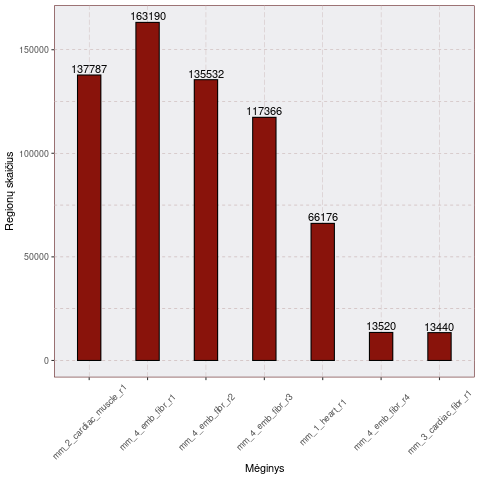
\includegraphics[width=0.7\linewidth]{Figures/total_peak_counts.png}
        \caption*{1 pav. Regionų skaičių kiekviename mėginyje vaizduojanti diagrama}
    \end{center}
\end{figure}

Remiantis diagrama didžiausias \emph{tbx5} transkripcijos faktoriaus
regionų skaičius nustatytas eksperimento \emph{(mm\_4\_emb\_fibr\_r1)}
biologinėje replikoje, kurioje pelių embrionų fibroblastų ląstelės
dvi dienas veiktos AGHMT faktoriais.
Šį rezultatą palyginus su kitomis biologinėmis replikomis, kuriose
tirtas tas pats pelių embrionų fibroblastų ląstelių kamienas, tačiau
ląstelės veiktos tik kai kuriais faktoriais, pastebimas gradualus
\emph{tbx5} transkripcijos faktoriaus regionų skaičiaus mažėjimas
diagramoje \emph{mm\_4\_emb\_fibr\_r2}, \emph{mm\_4\_emb\_fibr\_r3} ir
\emph{mm\_4\_emb\_fibr\_r4} pavaizduotuose stulpeliuose. Mėginyje,
kuriame embrionų fibroblastai veikti tik vienu faktoriumi,
\emph{tbx5} transkripcijos faktoriaus regionų nustatoma nedaug -
13520.

Tai leidžia daryti išvadą, kad \emph{tbx5} transkripcijos faktoriaus
geno ekspresija priklauso nuo kardiogeninių faktorių buvimo.

Mažiausiai regionų nustatyta mėginyje, kuriame tirta pelių
naujagimių širdies fibroblastų, ekspresuojančių T antigeną
ir paveiktų inhibitoriais: \emph{sb431542} ir \emph{xav939}.
Nepaisant to, kad abu inhibitoriai skatina širdies ląstelių
diferenciaciją, itin mažas transkripcijos faktoriaus regionų
skaičius rodo, kad papildomas veikimas inhibitoriais daro
mažą įtaką transkripcijos faktoriaus pasireiškimui.

\newpage

%%%%%%%%%%%%%%%%%%%%%%%%%%%%%%%%%%%%%%%%%%%%%
% REGIONŲ SKAIČIUS ATSKIROSE CHROMOSOMOSE
%%%%%%%%%%%%%%%%%%%%%%%%%%%%%%%%%%%%%%%%%%%%%
\subsection{Regionų pasiskirstymas chromosomose}
Nustačius \emph{tbx5} transkripcijos faktoriaus regionų
pasiskirstymą eksperimentų mėginiuose, kitame analizės etape
patikrinta, kaip faktoriaus regionai pasiskirstę atskirose
chromosomose.

Vaizduojamuose grafikuose didžiausias regionų skaičius nustatomas
pirmoje, antroje ir penktoje chromosomose. Naminės pelės pirmoji
chromosoma yra pati didžiausia, turinti 195 milijonų bazių porų,
antroji chromosoma sudaryta iš 182 megabazių, penktoji chromosoma -
152 milijonų bazių porų, todėl didesnis regionų skaičius šiose
chromosomose yra įprastas. Kitose chromosomose regionų skaičius
yra mažesnis. Ypač mažas regionų skaičius nustatomas devynioliktoje
(61 Mbp), X (169 Mbp) ir Y (91 Mbp) chromosomose.

Biologinių replikų mėginiuose didžiausias regionų skaičius
nustatytas antroje chromosomoje. Taip pat grafikuose išsiskiria
kontrolinis HL - 1 širdies ląstelių mėginys, kuriame didžiausias
regionų skaičius nustatomas penktojoje chromosomoje.

\begin{figure}[htb]
    \begin{center}
        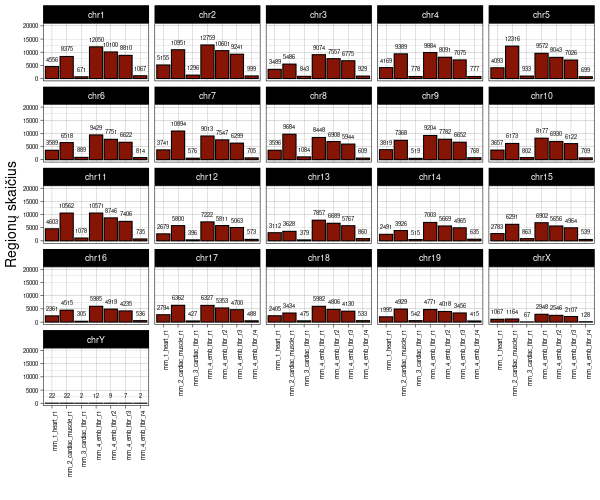
\includegraphics[width=0.8\linewidth]{Figures/peak_counts_by_chromosome.png}
        \caption*{2 pav. Regionų pasiskirstymas chromosomose}
    \end{center}
\end{figure}

\newpage

%%%%%%%%%%%%%%%%%%%%%%%%%%%%%%%%%%%%%%%%%%%%
% TARP MĖGINIŲ PERSIDENGIANTYS REGIONAI
%%%%%%%%%%%%%%%%%%%%%%%%%%%%%%%%%%%%%%%%%%%%
\subsection{Tarp mėginių persidengiantys regionai}
Dažnai siekiant nustatyti mėginių panašumą, yra tiriama, kokia
mėginių duomenų dalis persidengia.

\begin{figure}[htb]
    \begin{center}
        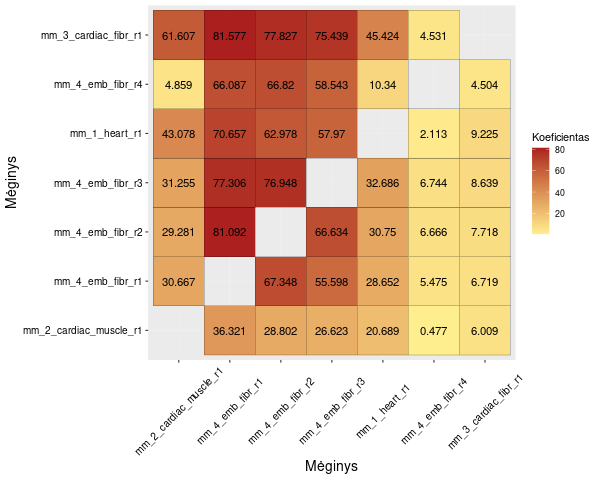
\includegraphics[width=0.8\linewidth]{Figures/peak_overlaps_between_samples.png}
        \caption*{3 pav. Persidengiančių regionų procentinės dalies vaizdavimas}
    \end{center}
\end{figure}

Remiantis pavaizduoto spalvų intensyvumo grafiko duomenimis,
didžiausiausi persidengiančių regionų procentai nustatyti tarp
šių mėginių:
\begin{itemize}
    \item \textbf{81.577 \%} - tarp mėginio, kuriame buvo tiriamos širdies
            fibroblastų ląstelės, ekspresuojančios T antigeną, ir pirmos
            biologinės replikos, kurioje tirti embrionų fibroblastai,
            veikiant AGHMT.
    \item \textbf{81.092 \%} - tarp pirmos biologinės replikos ir antros
            biologinės replikos, kurioje nebuvo AKT1.
    \item \textbf{77.827 \%} - tarp mėginio su T antigeną ekspresuojančiomis
            širdies fibroblastų ląstelėmis ir antros biologinės replikos.
    \item \textbf{76.948 \%} - tarp trečios biologinės replikos, kurioje
            nebuvo HAND2 faktoriaus, ir antros biologinės replikos.
    \item \textbf{75.439 \%} - tarp mėginio su T antigeną ekspresuojančiomis
            širdies fibroblastų ląstelėmis ir trečios biologinės replikomis.
  \end{itemize}

\newpage


% mm3_cardiac_fibr_r1 ir mm4_emb_fibr_r1
% mm4_emb_fibr_r1 ir mm4_emb_fibr_r2
% mm3_cardiac_fibr_r1 ir mm4_emb_fibr_r2
% mm4_emb_fibr_r3 ir mm4_emb_fibr_r2
% mm3_cardiac_fibr_r1 ir mm4_emb_fibr_r3

%%%%%%%%%%%%%%%%%%%%%%%%%%%%%%%%%%%%%%%%
% LITERATŪROS ŠALTINIAI
%%%%%%%%%%%%%%%%%%%%%%%%%%%%%%%%%%%%%%%%

\bibliographystyle{plain}
\begin{thebibliography}{99}
% \emph{bigBedToBed} aprašymas: https://genome.ucsc.edu/goldenPath/help/bigBed.html
% \emph{BEDTools} paketo dokumentacija: https://bedtools.readthedocs.io/en/latest/content/bedtools-suite.html
% \emph{getfasta} funkcijos dokumentacija: https://bedtools.readthedocs.io/en/latest/content/tools/getfasta.html
\end{thebibliography}
\newpage

%%%%%%%%%%%%%%%%%%%%%%%%%%%%%%%%%%%%%%%%
% PRIEDAI
%%%%%%%%%%%%%%%%%%%%%%%%%%%%%%%%%%%%%%%%

\section{Priedas}

\end{document}
